%\chapter{The Basics of Loading and Manipulating Data}
\chapter{Taxonomies of the Profane – Variables, Scales, and Their Unholy Properties}

\IMFellEnglish
\lettrine[lines=5, realheight]{T}{HERE} is a kind of grim devilry in the act of classification. The moment you categorize a thing—whether it be a small volume of blood, the reaction time of a startle, or the flickering presence of a belief—you strip it from the chaos of the unknown and chain it down, trembling, to a scale. Statisticians call them variables, but do not be fooled: these are not gentle creatures. They are twisted reflections of reality that must be bound in measurement and tortured into obedience. Nominal. Ordinal. Interval. Ratio. These are the sigils we etch into our grimoires of data, each one whispering what kind of rituals—summations, correlations, regressions—we may dare perform. But beware: misuse the wrong scale, or confuse the nature of your variable, and the results may turn on you, distorted and cursed. This chapter delves into the infernal art of measurement, uncovering the hidden laws that govern how data can be named, ranked, counted, or quantified. Prepare yourself—for to wield statistics is to practice a kind of taxonomy, yes  ... but one written in the ink of madness, precision, and utter cruelty.

\normalfont

\section{A Practical Problem}

Consider the complete craniometric dataset provided by  \textcite{Thomson1905}, available in the file \R{Thomson\_Randall-MacIver\_1905.csv},\footnote{The data file can be obtained at this book's GitHub repository: \url{https://github.com/statistical-grimoire/book/blob/main/data/Egyptian-skulls}} a ``small'' excerpt of which is displayed in Table \ref{tab:skulls_full}. The file contains a wide range of craniometric measurements along with other useful, and sometimes missing, contextual information, such as the estimated date range for each skull, the ruling dynasty at the time, and the archaeological site of origin. 

%\begin{landscape}
\begin{table}[p]
\centering
\resizebox{\textwidth}{!}{
\begin{tabular}{rrrlllllrrrrrrrrrrrrrlr}
\toprule
table & start\_date & end\_date & start\_era & end\_era & dynasty & location & sex & gol & ool & bbh & mb & biaurb & bizygb & bnl & bal & nah & nh & nw & fai & ga & po & cc\\
\midrule
\cellcolor{gray!10}{1} & \cellcolor{gray!10}{} & \cellcolor{gray!10}{} & \cellcolor{gray!10}{BC} & \cellcolor{gray!10}{BC} & \cellcolor{gray!10}{Early Predynastic} & \cellcolor{gray!10}{Abydos} & \cellcolor{gray!10}{Male} & \cellcolor{gray!10}{178.0} & \cellcolor{gray!10}{177} & \cellcolor{gray!10}{138.0} & \cellcolor{gray!10}{131} & \cellcolor{gray!10}{113} & \cellcolor{gray!10}{120.0} & \cellcolor{gray!10}{98} & \cellcolor{gray!10}{89} & \cellcolor{gray!10}{68.0} & \cellcolor{gray!10}{49} & \cellcolor{gray!10}{23.0} & \cellcolor{gray!10}{91.0} & \cellcolor{gray!10}{76.0} & \cellcolor{gray!10}{A} & \cellcolor{gray!10}{1370}\\
1 &  &  & BC & BC & Early Predynastic & Abydos & Male & 179.0 & 179 & 131.0 & 125 & 111 & 121.0 & 97 & 92 & 67.0 & 48 & 23.0 & 95.0 & 73.0 & B & 1250\\
\cellcolor{gray!10}{1} & \cellcolor{gray!10}{} & \cellcolor{gray!10}{} & \cellcolor{gray!10}{BC} & \cellcolor{gray!10}{BC} & \cellcolor{gray!10}{Early Predynastic} & \cellcolor{gray!10}{Abydos} & \cellcolor{gray!10}{Male} & \cellcolor{gray!10}{185.0} & \cellcolor{gray!10}{185} & \cellcolor{gray!10}{134.0} & \cellcolor{gray!10}{136} & \cellcolor{gray!10}{112} & \cellcolor{gray!10}{116.0} & \cellcolor{gray!10}{} & \cellcolor{gray!10}{} & \cellcolor{gray!10}{68.0} & \cellcolor{gray!10}{47} & \cellcolor{gray!10}{24.0} & \cellcolor{gray!10}{} & \cellcolor{gray!10}{} & \cellcolor{gray!10}{} & \cellcolor{gray!10}{1430}\\
1 &  &  & BC & BC & Early Predynastic & Abydos & Male & 183.0 & 180 & 132.0 & 131 & 112 & 122.0 & 103 & 99 & 64.0 & 50 & 26.0 & 96.0 & 74.5 & C & 1350\\
\cellcolor{gray!10}{1} & \cellcolor{gray!10}{} & \cellcolor{gray!10}{} & \cellcolor{gray!10}{BC} & \cellcolor{gray!10}{BC} & \cellcolor{gray!10}{Early Predynastic} & \cellcolor{gray!10}{Abydos} & \cellcolor{gray!10}{Male} & \cellcolor{gray!10}{169.0} & \cellcolor{gray!10}{169} & \cellcolor{gray!10}{132.0} & \cellcolor{gray!10}{119} & \cellcolor{gray!10}{106} & \cellcolor{gray!10}{119.0} & \cellcolor{gray!10}{100} & \cellcolor{gray!10}{96} & \cellcolor{gray!10}{64.0} & \cellcolor{gray!10}{44} & \cellcolor{gray!10}{25.0} & \cellcolor{gray!10}{96.0} & \cellcolor{gray!10}{74.0} & \cellcolor{gray!10}{B C} & \cellcolor{gray!10}{1130}\\
\addlinespace
1 &  &  & BC & BC & Early Predynastic & Abydos & Male & 202.0 & 202 & 143.0 & 136 & 119 & 130.0 & 107 & 100 & 75.0 & 54 & 24.0 & 93.0 & 73.5 & A & 1670\\
\cellcolor{gray!10}{1} & \cellcolor{gray!10}{} & \cellcolor{gray!10}{} & \cellcolor{gray!10}{BC} & \cellcolor{gray!10}{BC} & \cellcolor{gray!10}{Early Predynastic} & \cellcolor{gray!10}{Abydos} & \cellcolor{gray!10}{Male} & \cellcolor{gray!10}{185.0} & \cellcolor{gray!10}{185} & \cellcolor{gray!10}{} & \cellcolor{gray!10}{114} & \cellcolor{gray!10}{} & \cellcolor{gray!10}{} & \cellcolor{gray!10}{} & \cellcolor{gray!10}{} & \cellcolor{gray!10}{68.0} & \cellcolor{gray!10}{47} & \cellcolor{gray!10}{23.0} & \cellcolor{gray!10}{} & \cellcolor{gray!10}{} & \cellcolor{gray!10}{} & \cellcolor{gray!10}{}\\
1 &  &  & BC & BC & Early Predynastic & Abydos & Male & 175.0 & 175 &  & 128 &  &  &  &  &  &  &  &  &  &  & \\
\cellcolor{gray!10}{1} & \cellcolor{gray!10}{} & \cellcolor{gray!10}{} & \cellcolor{gray!10}{BC} & \cellcolor{gray!10}{BC} & \cellcolor{gray!10}{Early Predynastic} & \cellcolor{gray!10}{Abydos} & \cellcolor{gray!10}{Male} & \cellcolor{gray!10}{190.0} & \cellcolor{gray!10}{190} & \cellcolor{gray!10}{} & \cellcolor{gray!10}{146} & \cellcolor{gray!10}{} & \cellcolor{gray!10}{} & \cellcolor{gray!10}{} & \cellcolor{gray!10}{} & \cellcolor{gray!10}{} & \cellcolor{gray!10}{} & \cellcolor{gray!10}{} & \cellcolor{gray!10}{} & \cellcolor{gray!10}{} & \cellcolor{gray!10}{} & \cellcolor{gray!10}{}\\
1 &  &  & BC & BC & Early Predynastic & Abydos & Male & 188.0 & 188 &  & 127 &  &  &  &  &  &  &  &  &  &  & \\
\addlinespace
\cellcolor{gray!10}{1} & \cellcolor{gray!10}{} & \cellcolor{gray!10}{} & \cellcolor{gray!10}{BC} & \cellcolor{gray!10}{BC} & \cellcolor{gray!10}{Early Predynastic} & \cellcolor{gray!10}{Abydos} & \cellcolor{gray!10}{Male} & \cellcolor{gray!10}{177.0} & \cellcolor{gray!10}{177} & \cellcolor{gray!10}{122.0} & \cellcolor{gray!10}{130} & \cellcolor{gray!10}{} & \cellcolor{gray!10}{} & \cellcolor{gray!10}{} & \cellcolor{gray!10}{} & \cellcolor{gray!10}{} & \cellcolor{gray!10}{} & \cellcolor{gray!10}{} & \cellcolor{gray!10}{} & \cellcolor{gray!10}{} & \cellcolor{gray!10}{} & \cellcolor{gray!10}{1195}\\
1 &  &  & BC & BC & Early Predynastic & Abydos & Male & 192.0 & 189 &  & 136 &  &  &  &  &  &  &  &  &  &  & \\
\cellcolor{gray!10}{1} & \cellcolor{gray!10}{} & \cellcolor{gray!10}{} & \cellcolor{gray!10}{BC} & \cellcolor{gray!10}{BC} & \cellcolor{gray!10}{Early Predynastic} & \cellcolor{gray!10}{Abydos} & \cellcolor{gray!10}{Male} & \cellcolor{gray!10}{187.0} & \cellcolor{gray!10}{187} & \cellcolor{gray!10}{137.0} & \cellcolor{gray!10}{138} & \cellcolor{gray!10}{114} & \cellcolor{gray!10}{123.0} & \cellcolor{gray!10}{96} & \cellcolor{gray!10}{89} & \cellcolor{gray!10}{76.0} & \cellcolor{gray!10}{56} & \cellcolor{gray!10}{25.0} & \cellcolor{gray!10}{93.0} & \cellcolor{gray!10}{70.5} & \cellcolor{gray!10}{A} & \cellcolor{gray!10}{1500}\\
1 &  &  & BC & BC & Early Predynastic & Abydos & Male & 176.0 & 174 & 134.0 & 132 & 100 &  & 98 & 86 & 65.0 &  &  & 88.0 & 79.5 & - A & 1325\\
\cellcolor{gray!10}{1} & \cellcolor{gray!10}{} & \cellcolor{gray!10}{} & \cellcolor{gray!10}{BC} & \cellcolor{gray!10}{BC} & \cellcolor{gray!10}{Early Predynastic} & \cellcolor{gray!10}{Abydos} & \cellcolor{gray!10}{Male} & \cellcolor{gray!10}{192.0} & \cellcolor{gray!10}{192} & \cellcolor{gray!10}{130.0} & \cellcolor{gray!10}{139} & \cellcolor{gray!10}{115} & \cellcolor{gray!10}{125.0} & \cellcolor{gray!10}{103} & \cellcolor{gray!10}{108} & \cellcolor{gray!10}{72.0} & \cellcolor{gray!10}{48} & \cellcolor{gray!10}{28.0} & \cellcolor{gray!10}{105.0} & \cellcolor{gray!10}{66.0} & \cellcolor{gray!10}{E F} & \cellcolor{gray!10}{1480}\\
\addlinespace
1 &  &  & BC & BC & Early Predynastic & Abydos & Male & 187.0 & 187 &  & 132 &  &  &  &  &  &  &  &  &  &  & \\
\cellcolor{gray!10}{1} & \cellcolor{gray!10}{} & \cellcolor{gray!10}{} & \cellcolor{gray!10}{BC} & \cellcolor{gray!10}{BC} & \cellcolor{gray!10}{Early Predynastic} & \cellcolor{gray!10}{Abydos} & \cellcolor{gray!10}{Male} & \cellcolor{gray!10}{187.0} & \cellcolor{gray!10}{185} & \cellcolor{gray!10}{136.0} & \cellcolor{gray!10}{125} & \cellcolor{gray!10}{105} & \cellcolor{gray!10}{119.0} & \cellcolor{gray!10}{101} & \cellcolor{gray!10}{93} & \cellcolor{gray!10}{66.0} & \cellcolor{gray!10}{48} & \cellcolor{gray!10}{25.0} & \cellcolor{gray!10}{92.0} & \cellcolor{gray!10}{76.0} & \cellcolor{gray!10}{A} & \cellcolor{gray!10}{1350}\\
1 &  &  & BC & BC & Early Predynastic & Abydos & Male & 181.0 & 177 & 134.0 & 131 & 112 & 125.0 & 102 & 102 & 76.0 & 51 & 25.0 & 100.0 & 68.0 & C & 1350\\
\cellcolor{gray!10}{1} & \cellcolor{gray!10}{} & \cellcolor{gray!10}{} & \cellcolor{gray!10}{BC} & \cellcolor{gray!10}{BC} & \cellcolor{gray!10}{Early Predynastic} & \cellcolor{gray!10}{Abydos} & \cellcolor{gray!10}{Male} & \cellcolor{gray!10}{194.0} & \cellcolor{gray!10}{191} & \cellcolor{gray!10}{134.0} & \cellcolor{gray!10}{134} & \cellcolor{gray!10}{127} & \cellcolor{gray!10}{} & \cellcolor{gray!10}{109} & \cellcolor{gray!10}{99} & \cellcolor{gray!10}{72.0} & \cellcolor{gray!10}{51} & \cellcolor{gray!10}{26.0} & \cellcolor{gray!10}{91.0} & \cellcolor{gray!10}{77.5} & \cellcolor{gray!10}{A} & \cellcolor{gray!10}{1480}\\
1 &  &  & BC & BC & Early Predynastic & Abydos & Male & 191.0 & 189 &  & 130 &  &  &  &  &  &  &  &  &  &  & \\
\addlinespace
\cellcolor{gray!10}{1} & \cellcolor{gray!10}{} & \cellcolor{gray!10}{} & \cellcolor{gray!10}{BC} & \cellcolor{gray!10}{BC} & \cellcolor{gray!10}{Early Predynastic} & \cellcolor{gray!10}{EL Amrah} & \cellcolor{gray!10}{Male} & \cellcolor{gray!10}{161.0} & \cellcolor{gray!10}{161} & \cellcolor{gray!10}{} & \cellcolor{gray!10}{129} & \cellcolor{gray!10}{} & \cellcolor{gray!10}{} & \cellcolor{gray!10}{} & \cellcolor{gray!10}{} & \cellcolor{gray!10}{} & \cellcolor{gray!10}{} & \cellcolor{gray!10}{} & \cellcolor{gray!10}{} & \cellcolor{gray!10}{} & \cellcolor{gray!10}{} & \cellcolor{gray!10}{}\\
1 &  &  & BC & BC & Early Predynastic & EL Amrah & Male & 181.0 & 180 & 138.0 & 129 &  & 123.0 & 106 & 95 & 65.0 & 50 & 24.0 & 90.0 & 80.0 & A & 1370\\
\cellcolor{gray!10}{1} & \cellcolor{gray!10}{} & \cellcolor{gray!10}{} & \cellcolor{gray!10}{BC} & \cellcolor{gray!10}{BC} & \cellcolor{gray!10}{Early Predynastic} & \cellcolor{gray!10}{EL Amrah} & \cellcolor{gray!10}{Male} & \cellcolor{gray!10}{188.0} & \cellcolor{gray!10}{188} & \cellcolor{gray!10}{138.0} & \cellcolor{gray!10}{135} & \cellcolor{gray!10}{} & \cellcolor{gray!10}{113.0} & \cellcolor{gray!10}{} & \cellcolor{gray!10}{} & \cellcolor{gray!10}{67.0} & \cellcolor{gray!10}{47} & \cellcolor{gray!10}{26.0} & \cellcolor{gray!10}{} & \cellcolor{gray!10}{} & \cellcolor{gray!10}{} & \cellcolor{gray!10}{1490}\\
1 &  &  & BC & BC & Early Predynastic & EL Amrah & Male & 169.0 &  &  & 140 &  &  &  &  &  &  &  &  &  &  & \\
\cellcolor{gray!10}{1} & \cellcolor{gray!10}{} & \cellcolor{gray!10}{} & \cellcolor{gray!10}{BC} & \cellcolor{gray!10}{BC} & \cellcolor{gray!10}{Early Predynastic} & \cellcolor{gray!10}{EL Amrah} & \cellcolor{gray!10}{Male} & \cellcolor{gray!10}{189.0} & \cellcolor{gray!10}{188} & \cellcolor{gray!10}{} & \cellcolor{gray!10}{138} & \cellcolor{gray!10}{} & \cellcolor{gray!10}{} & \cellcolor{gray!10}{} & \cellcolor{gray!10}{} & \cellcolor{gray!10}{} & \cellcolor{gray!10}{} & \cellcolor{gray!10}{} & \cellcolor{gray!10}{} & \cellcolor{gray!10}{} & \cellcolor{gray!10}{} & \cellcolor{gray!10}{}\\
\addlinespace
1 &  &  & BC & BC & Early Predynastic & EL Amrah & Male & 189.0 & 189 &  & 125 &  &  &  &  &  &  &  &  &  &  & \\
\cellcolor{gray!10}{1} & \cellcolor{gray!10}{} & \cellcolor{gray!10}{} & \cellcolor{gray!10}{BC} & \cellcolor{gray!10}{BC} & \cellcolor{gray!10}{Early Predynastic} & \cellcolor{gray!10}{EL Amrah} & \cellcolor{gray!10}{Male} & \cellcolor{gray!10}{182.0} & \cellcolor{gray!10}{184} & \cellcolor{gray!10}{} & \cellcolor{gray!10}{128} & \cellcolor{gray!10}{} & \cellcolor{gray!10}{} & \cellcolor{gray!10}{} & \cellcolor{gray!10}{} & \cellcolor{gray!10}{} & \cellcolor{gray!10}{} & \cellcolor{gray!10}{} & \cellcolor{gray!10}{} & \cellcolor{gray!10}{} & \cellcolor{gray!10}{} & \cellcolor{gray!10}{}\\
1 &  &  & BC & BC & Early Predynastic & EL Amrah & Male & 195.0 & 193 &  &  &  &  &  &  &  &  &  &  &  &  & \\
\cellcolor{gray!10}{1} & \cellcolor{gray!10}{} & \cellcolor{gray!10}{} & \cellcolor{gray!10}{BC} & \cellcolor{gray!10}{BC} & \cellcolor{gray!10}{Early Predynastic} & \cellcolor{gray!10}{EL Amrah} & \cellcolor{gray!10}{Male} & \cellcolor{gray!10}{193.0} & \cellcolor{gray!10}{191} & \cellcolor{gray!10}{140.5} & \cellcolor{gray!10}{131} & \cellcolor{gray!10}{} & \cellcolor{gray!10}{128.0} & \cellcolor{gray!10}{} & \cellcolor{gray!10}{} & \cellcolor{gray!10}{} & \cellcolor{gray!10}{} & \cellcolor{gray!10}{} & \cellcolor{gray!10}{} & \cellcolor{gray!10}{} & \cellcolor{gray!10}{} & \cellcolor{gray!10}{1495}\\
1 &  &  & BC & BC & Early Predynastic & EL Amrah & Male & 190.0 & 188 &  & 125 &  &  &  &  &  &  &  &  &  &  & \\
\addlinespace
\cellcolor{gray!10}{1} & \cellcolor{gray!10}{} & \cellcolor{gray!10}{} & \cellcolor{gray!10}{BC} & \cellcolor{gray!10}{BC} & \cellcolor{gray!10}{Early Predynastic} & \cellcolor{gray!10}{Hou} & \cellcolor{gray!10}{Male} & \cellcolor{gray!10}{177.0} & \cellcolor{gray!10}{176} & \cellcolor{gray!10}{121.0} & \cellcolor{gray!10}{134} & \cellcolor{gray!10}{116} & \cellcolor{gray!10}{125.0} & \cellcolor{gray!10}{96} & \cellcolor{gray!10}{95} & \cellcolor{gray!10}{72.0} & \cellcolor{gray!10}{53} & \cellcolor{gray!10}{25.0} & \cellcolor{gray!10}{99.0} & \cellcolor{gray!10}{68.0} & \cellcolor{gray!10}{B C} & \cellcolor{gray!10}{1220}\\
1 &  &  & BC & BC & Early Predynastic & Hou & Male & 189.0 & 188 & 129.0 & 126 & 111 & 126.0 & 105 & 109 & 68.0 & 51 & 26.0 & 104.0 & 68.0 & F & 1305\\
\cellcolor{gray!10}{1} & \cellcolor{gray!10}{} & \cellcolor{gray!10}{} & \cellcolor{gray!10}{BC} & \cellcolor{gray!10}{BC} & \cellcolor{gray!10}{Early Predynastic} & \cellcolor{gray!10}{Hou} & \cellcolor{gray!10}{Male} & \cellcolor{gray!10}{190.0} & \cellcolor{gray!10}{188} & \cellcolor{gray!10}{142.0} & \cellcolor{gray!10}{133} & \cellcolor{gray!10}{114} & \cellcolor{gray!10}{} & \cellcolor{gray!10}{106} & \cellcolor{gray!10}{107} & \cellcolor{gray!10}{64.0} & \cellcolor{gray!10}{} & \cellcolor{gray!10}{} & \cellcolor{gray!10}{101.0} & \cellcolor{gray!10}{71.0} & \cellcolor{gray!10}{E} & \cellcolor{gray!10}{1525}\\
1 &  &  & BC & BC & Early Predynastic & Hou & Male & 180.0 & 179 & 136.0 & 132 & 121 & 129.0 & 102 & 100 & 66.0 & 50 & 27.0 & 98.0 & 72.0 & C D & 1375\\
\cellcolor{gray!10}{1} & \cellcolor{gray!10}{} & \cellcolor{gray!10}{} & \cellcolor{gray!10}{BC} & \cellcolor{gray!10}{BC} & \cellcolor{gray!10}{Early Predynastic} & \cellcolor{gray!10}{Hou} & \cellcolor{gray!10}{Male} & \cellcolor{gray!10}{181.0} & \cellcolor{gray!10}{179} & \cellcolor{gray!10}{140.0} & \cellcolor{gray!10}{141} & \cellcolor{gray!10}{114} & \cellcolor{gray!10}{125.0} & \cellcolor{gray!10}{102} & \cellcolor{gray!10}{100} & \cellcolor{gray!10}{72.0} & \cellcolor{gray!10}{51} & \cellcolor{gray!10}{27.0} & \cellcolor{gray!10}{98.0} & \cellcolor{gray!10}{70.0} & \cellcolor{gray!10}{C} & \cellcolor{gray!10}{1520}\\
\addlinespace
1 &  &  & BC & BC & Early Predynastic & Hou & Male & 174.0 & 171 & 134.0 & 131 & 116 & 130.0 & 99 & 97 & 69.0 & 54 & 22.0 & 98.0 & 71.0 & C & 1300\\
\cellcolor{gray!10}{1} & \cellcolor{gray!10}{} & \cellcolor{gray!10}{} & \cellcolor{gray!10}{BC} & \cellcolor{gray!10}{BC} & \cellcolor{gray!10}{Early Predynastic} & \cellcolor{gray!10}{Hou} & \cellcolor{gray!10}{Male} & \cellcolor{gray!10}{178.0} & \cellcolor{gray!10}{178} & \cellcolor{gray!10}{137.0} & \cellcolor{gray!10}{135} & \cellcolor{gray!10}{112} & \cellcolor{gray!10}{122.0} & \cellcolor{gray!10}{109} & \cellcolor{gray!10}{103} & \cellcolor{gray!10}{74.0} & \cellcolor{gray!10}{50} & \cellcolor{gray!10}{24.0} & \cellcolor{gray!10}{94.5} & \cellcolor{gray!10}{74.0} & \cellcolor{gray!10}{A B} & \cellcolor{gray!10}{1400}\\
1 &  &  & BC & BC & Early Predynastic & Hou & Male & 176.0 & 173 & 133.0 & 132 & 112 & 126.0 & 98 & 93 & 72.0 & 53 & 26.0 & 95.0 & 71.5 & A B & 1315\\
\cellcolor{gray!10}{1} & \cellcolor{gray!10}{} & \cellcolor{gray!10}{} & \cellcolor{gray!10}{BC} & \cellcolor{gray!10}{BC} & \cellcolor{gray!10}{Early Predynastic} & \cellcolor{gray!10}{Hou} & \cellcolor{gray!10}{Male} & \cellcolor{gray!10}{181.0} & \cellcolor{gray!10}{179} & \cellcolor{gray!10}{136.0} & \cellcolor{gray!10}{139} & \cellcolor{gray!10}{116} & \cellcolor{gray!10}{} & \cellcolor{gray!10}{98} & \cellcolor{gray!10}{96} & \cellcolor{gray!10}{70.0} & \cellcolor{gray!10}{50} & \cellcolor{gray!10}{27.0} & \cellcolor{gray!10}{98.0} & \cellcolor{gray!10}{70.0} & \cellcolor{gray!10}{} & \cellcolor{gray!10}{1460}\\
1 &  &  & BC & BC & Early Predynastic & Hou & Male & 185.0 & 183 & 131.0 & 132 & 111 & 124.0 & 104 & 101 & 68.0 & 49 & 26.0 & 97.0 & 73.0 & C & 1360\\
\addlinespace
\cellcolor{gray!10}{1} & \cellcolor{gray!10}{} & \cellcolor{gray!10}{} & \cellcolor{gray!10}{BC} & \cellcolor{gray!10}{BC} & \cellcolor{gray!10}{Early Predynastic} & \cellcolor{gray!10}{Hou} & \cellcolor{gray!10}{Male} & \cellcolor{gray!10}{184.0} & \cellcolor{gray!10}{184} & \cellcolor{gray!10}{133.0} & \cellcolor{gray!10}{126} & \cellcolor{gray!10}{114} & \cellcolor{gray!10}{125.0} & \cellcolor{gray!10}{103} & \cellcolor{gray!10}{102} & \cellcolor{gray!10}{66.0} & \cellcolor{gray!10}{51} & \cellcolor{gray!10}{28.0} & \cellcolor{gray!10}{99.0} & \cellcolor{gray!10}{72.0} & \cellcolor{gray!10}{D} & \cellcolor{gray!10}{1310}\\
2 &  &  & BC & BC & Early Predynastic & Hou & Male & 186.0 & 185 & 135.0 & 135 & 116 & 125.0 & 105 & 103 & 66.0 & 47 & 26.0 & 98.0 & 73.0 & D & 1440\\
\cellcolor{gray!10}{2} & \cellcolor{gray!10}{} & \cellcolor{gray!10}{} & \cellcolor{gray!10}{BC} & \cellcolor{gray!10}{BC} & \cellcolor{gray!10}{Early Predynastic} & \cellcolor{gray!10}{Hou} & \cellcolor{gray!10}{Male} & \cellcolor{gray!10}{176.0} & \cellcolor{gray!10}{175} & \cellcolor{gray!10}{124.0} & \cellcolor{gray!10}{134} & \cellcolor{gray!10}{110} & \cellcolor{gray!10}{123.0} & \cellcolor{gray!10}{96} & \cellcolor{gray!10}{93} & \cellcolor{gray!10}{74.0} & \cellcolor{gray!10}{53} & \cellcolor{gray!10}{23.0} & \cellcolor{gray!10}{97.0} & \cellcolor{gray!10}{69.0} & \cellcolor{gray!10}{A B} & \cellcolor{gray!10}{1245}\\
2 &  &  & BC & BC & Early Predynastic & Hou & Male & 187.0 & 186 & 134.0 & 128 &  &  & 110 & 103 & 67.0 & 50 & 27.0 & 94.0 & 77.0 & B C & 1360\\
\cellcolor{gray!10}{2} & \cellcolor{gray!10}{} & \cellcolor{gray!10}{} & \cellcolor{gray!10}{BC} & \cellcolor{gray!10}{BC} & \cellcolor{gray!10}{Early Predynastic} & \cellcolor{gray!10}{Hou} & \cellcolor{gray!10}{Male} & \cellcolor{gray!10}{181.0} & \cellcolor{gray!10}{181} & \cellcolor{gray!10}{130.0} & \cellcolor{gray!10}{130} & \cellcolor{gray!10}{117} & \cellcolor{gray!10}{129.0} & \cellcolor{gray!10}{103} & \cellcolor{gray!10}{104} & \cellcolor{gray!10}{69.0} & \cellcolor{gray!10}{49} & \cellcolor{gray!10}{25.0} & \cellcolor{gray!10}{101.0} & \cellcolor{gray!10}{69.5} & \cellcolor{gray!10}{D E} & \cellcolor{gray!10}{1300}\\
\addlinespace
2 &  &  & BC & BC & Early Predynastic & Hou & Male & 185.0 & 182 & 135.0 & 138 & 121 & 136.0 & 104 & 100 & 78.0 & 55 & 27.0 & 96.0 & 70.0 & A B & 1470\\
\cellcolor{gray!10}{2} & \cellcolor{gray!10}{} & \cellcolor{gray!10}{} & \cellcolor{gray!10}{BC} & \cellcolor{gray!10}{BC} & \cellcolor{gray!10}{Early Predynastic} & \cellcolor{gray!10}{Hou} & \cellcolor{gray!10}{Male} & \cellcolor{gray!10}{184.0} & \cellcolor{gray!10}{184} & \cellcolor{gray!10}{132.0} & \cellcolor{gray!10}{128} & \cellcolor{gray!10}{106} & \cellcolor{gray!10}{117.0} & \cellcolor{gray!10}{97} & \cellcolor{gray!10}{93} & \cellcolor{gray!10}{72.0} & \cellcolor{gray!10}{53} & \cellcolor{gray!10}{25.0} & \cellcolor{gray!10}{96.0} & \cellcolor{gray!10}{70.5} & \cellcolor{gray!10}{A B} & \cellcolor{gray!10}{1320}\\
2 &  &  & BC & BC & Early Predynastic & Hou & Male & 184.0 & 184 & 129.0 & 127 & 116 & 131.0 & 102 & 106 & 63.0 & 48 & 28.0 & 104.0 & 68.5 & F & 1290\\
\cellcolor{gray!10}{2} & \cellcolor{gray!10}{} & \cellcolor{gray!10}{} & \cellcolor{gray!10}{BC} & \cellcolor{gray!10}{BC} & \cellcolor{gray!10}{Early Predynastic} & \cellcolor{gray!10}{Hou} & \cellcolor{gray!10}{Male} & \cellcolor{gray!10}{185.0} & \cellcolor{gray!10}{183} & \cellcolor{gray!10}{136.0} & \cellcolor{gray!10}{131} & \cellcolor{gray!10}{117} & \cellcolor{gray!10}{129.0} & \cellcolor{gray!10}{111} & \cellcolor{gray!10}{114} & \cellcolor{gray!10}{73.0} & \cellcolor{gray!10}{54} & \cellcolor{gray!10}{27.0} & \cellcolor{gray!10}{103.0} & \cellcolor{gray!10}{68.5} & \cellcolor{gray!10}{E F} & \cellcolor{gray!10}{1400}\\
2 &  &  & BC & BC & Early Predynastic & Hou & Male & 180.0 & 179 & 138.0 & 124 & 114 & 120.0 & 101 & 101 & 62.0 & 46 & 25.0 & 100.0 & 71.5 & D E & 1310\\
\addlinespace
\cellcolor{gray!10}{2} & \cellcolor{gray!10}{} & \cellcolor{gray!10}{} & \cellcolor{gray!10}{BC} & \cellcolor{gray!10}{BC} & \cellcolor{gray!10}{Early Predynastic} & \cellcolor{gray!10}{Hou} & \cellcolor{gray!10}{Male} & \cellcolor{gray!10}{181.0} & \cellcolor{gray!10}{180} & \cellcolor{gray!10}{139.0} & \cellcolor{gray!10}{131} & \cellcolor{gray!10}{113} & \cellcolor{gray!10}{121.0} & \cellcolor{gray!10}{98} & \cellcolor{gray!10}{92} & \cellcolor{gray!10}{71.0} & \cellcolor{gray!10}{53} & \cellcolor{gray!10}{24.0} & \cellcolor{gray!10}{94.0} & \cellcolor{gray!10}{73.0} & \cellcolor{gray!10}{A} & \cellcolor{gray!10}{1400}\\
2 &  &  & BC & BC & Early Predynastic & Hou & Male & 183.0 & 182 & 138.0 & 131 & 111 & 126.0 & 102 & 98 & 73.0 & 49 & 24.0 & 96.0 & 71.0 & B & 1410\\
\cellcolor{gray!10}{2} & \cellcolor{gray!10}{} & \cellcolor{gray!10}{} & \cellcolor{gray!10}{BC} & \cellcolor{gray!10}{BC} & \cellcolor{gray!10}{Early Predynastic} & \cellcolor{gray!10}{Hou} & \cellcolor{gray!10}{Male} & \cellcolor{gray!10}{183.0} & \cellcolor{gray!10}{180} & \cellcolor{gray!10}{140.0} & \cellcolor{gray!10}{137} & \cellcolor{gray!10}{127} & \cellcolor{gray!10}{133.0} & \cellcolor{gray!10}{103} & \cellcolor{gray!10}{103} & \cellcolor{gray!10}{74.0} & \cellcolor{gray!10}{52} & \cellcolor{gray!10}{22.0} & \cellcolor{gray!10}{100.0} & \cellcolor{gray!10}{69.0} & \cellcolor{gray!10}{C} & \cellcolor{gray!10}{1495}\\
2 &  &  & BC & BC & Early Predynastic & Hou & Male & 184.0 & 180 & 125.0 & 128 & 112 & 121.0 & 98 & 95 & 64.0 & 44 & 24.0 & 97.0 & 72.5 & C & 1250\\
\cellcolor{gray!10}{2} & \cellcolor{gray!10}{} & \cellcolor{gray!10}{} & \cellcolor{gray!10}{BC} & \cellcolor{gray!10}{BC} & \cellcolor{gray!10}{Late Predynastic} & \cellcolor{gray!10}{El Amrah} & \cellcolor{gray!10}{Male} & \cellcolor{gray!10}{185.0} & \cellcolor{gray!10}{185} & \cellcolor{gray!10}{138.0} & \cellcolor{gray!10}{124} & \cellcolor{gray!10}{115} & \cellcolor{gray!10}{122.0} & \cellcolor{gray!10}{102} & \cellcolor{gray!10}{101} & \cellcolor{gray!10}{67.0} & \cellcolor{gray!10}{48} & \cellcolor{gray!10}{26.0} & \cellcolor{gray!10}{99.0} & \cellcolor{gray!10}{71.0} & \cellcolor{gray!10}{D} & \cellcolor{gray!10}{1350}\\
\addlinespace
2 &  &  & BC & BC & Late Predynastic & El Amrah & Male & 178.0 & 176 &  & 138 &  &  &  &  &  &  &  &  &  &  & \\
\cellcolor{gray!10}{2} & \cellcolor{gray!10}{} & \cellcolor{gray!10}{} & \cellcolor{gray!10}{BC} & \cellcolor{gray!10}{BC} & \cellcolor{gray!10}{Late Predynastic} & \cellcolor{gray!10}{El Amrah} & \cellcolor{gray!10}{Male} & \cellcolor{gray!10}{189.0} & \cellcolor{gray!10}{187} & \cellcolor{gray!10}{134.0} & \cellcolor{gray!10}{133} & \cellcolor{gray!10}{} & \cellcolor{gray!10}{129.0} & \cellcolor{gray!10}{99} & \cellcolor{gray!10}{97} & \cellcolor{gray!10}{65.0} & \cellcolor{gray!10}{48} & \cellcolor{gray!10}{30.0} & \cellcolor{gray!10}{98.0} & \cellcolor{gray!10}{72.0} & \cellcolor{gray!10}{C D} & \cellcolor{gray!10}{1430}\\
2 &  &  & BC & BC & Late Predynastic & El Amrah & Male & 183.0 & 182 &  & 142 &  &  &  &  &  &  &  &  &  &  & \\
\cellcolor{gray!10}{2} & \cellcolor{gray!10}{} & \cellcolor{gray!10}{} & \cellcolor{gray!10}{BC} & \cellcolor{gray!10}{BC} & \cellcolor{gray!10}{Late Predynastic} & \cellcolor{gray!10}{El Amrah} & \cellcolor{gray!10}{Male} & \cellcolor{gray!10}{183.0} & \cellcolor{gray!10}{183} & \cellcolor{gray!10}{} & \cellcolor{gray!10}{141} & \cellcolor{gray!10}{} & \cellcolor{gray!10}{} & \cellcolor{gray!10}{} & \cellcolor{gray!10}{} & \cellcolor{gray!10}{} & \cellcolor{gray!10}{} & \cellcolor{gray!10}{} & \cellcolor{gray!10}{} & \cellcolor{gray!10}{} & \cellcolor{gray!10}{} & \cellcolor{gray!10}{}\\
2 &  &  & BC & BC & Late Predynastic & El Amrah & Male & 194.0 & 194 &  & 134 &  &  &  &  &  &  &  &  &  &  & \\
\addlinespace
\cellcolor{gray!10}{2} & \cellcolor{gray!10}{} & \cellcolor{gray!10}{} & \cellcolor{gray!10}{BC} & \cellcolor{gray!10}{BC} & \cellcolor{gray!10}{Late Predynastic} & \cellcolor{gray!10}{El Amrah} & \cellcolor{gray!10}{Male} & \cellcolor{gray!10}{189.0} & \cellcolor{gray!10}{189} & \cellcolor{gray!10}{134.0} & \cellcolor{gray!10}{138} & \cellcolor{gray!10}{} & \cellcolor{gray!10}{120.0} & \cellcolor{gray!10}{100} & \cellcolor{gray!10}{98} & \cellcolor{gray!10}{67.0} & \cellcolor{gray!10}{45} & \cellcolor{gray!10}{26.0} & \cellcolor{gray!10}{98.0} & \cellcolor{gray!10}{71.0} & \cellcolor{gray!10}{C} & \cellcolor{gray!10}{1490}\\
2 &  &  & BC & BC & Late Predynastic & El Amrah & Male & 190.0 & 190 &  & 132 &  &  &  &  &  &  &  &  &  &  & \\
\cellcolor{gray!10}{2} & \cellcolor{gray!10}{} & \cellcolor{gray!10}{} & \cellcolor{gray!10}{BC} & \cellcolor{gray!10}{BC} & \cellcolor{gray!10}{Late Predynastic} & \cellcolor{gray!10}{El Amrah} & \cellcolor{gray!10}{Male} & \cellcolor{gray!10}{190.0} & \cellcolor{gray!10}{186} & \cellcolor{gray!10}{129.0} & \cellcolor{gray!10}{148} & \cellcolor{gray!10}{130} & \cellcolor{gray!10}{134.0} & \cellcolor{gray!10}{100} & \cellcolor{gray!10}{104} & \cellcolor{gray!10}{69.0} & \cellcolor{gray!10}{51} & \cellcolor{gray!10}{24.0} & \cellcolor{gray!10}{} & \cellcolor{gray!10}{} & \cellcolor{gray!10}{} & \cellcolor{gray!10}{}\\
2 &  &  & BC & BC & Late Predynastic & El Amrah & Male & 172.0 & 171 & 124.0 & 126 & 110 & 117.0 & 98 & 95 & 61.0 & 45 & 27.0 & 97.0 & 74.0 & C D & 1140\\
\cellcolor{gray!10}{2} & \cellcolor{gray!10}{} & \cellcolor{gray!10}{} & \cellcolor{gray!10}{BC} & \cellcolor{gray!10}{BC} & \cellcolor{gray!10}{Late Predynastic} & \cellcolor{gray!10}{El Amrah} & \cellcolor{gray!10}{Male} & \cellcolor{gray!10}{191.0} & \cellcolor{gray!10}{187} & \cellcolor{gray!10}{136.0} & \cellcolor{gray!10}{135} & \cellcolor{gray!10}{115} & \cellcolor{gray!10}{128.0} & \cellcolor{gray!10}{104} & \cellcolor{gray!10}{98} & \cellcolor{gray!10}{71.0} & \cellcolor{gray!10}{52} & \cellcolor{gray!10}{25.0} & \cellcolor{gray!10}{94.0} & \cellcolor{gray!10}{74.0} & \cellcolor{gray!10}{A B} & \cellcolor{gray!10}{1490}\\
\addlinespace
2 &  &  & BC & BC & Late Predynastic & El Amrah & Male & 185.0 & 184 & 145.0 & 132 & 119 & 130.0 & 102 & 100 & 71.0 & 54 & 23.0 & 98.0 & 70.5 & C & 1505\\
\cellcolor{gray!10}{2} & \cellcolor{gray!10}{} & \cellcolor{gray!10}{} & \cellcolor{gray!10}{BC} & \cellcolor{gray!10}{BC} & \cellcolor{gray!10}{Late Predynastic} & \cellcolor{gray!10}{El Amrah} & \cellcolor{gray!10}{Male} & \cellcolor{gray!10}{187.0} & \cellcolor{gray!10}{185} & \cellcolor{gray!10}{} & \cellcolor{gray!10}{134} & \cellcolor{gray!10}{} & \cellcolor{gray!10}{} & \cellcolor{gray!10}{} & \cellcolor{gray!10}{} & \cellcolor{gray!10}{} & \cellcolor{gray!10}{} & \cellcolor{gray!10}{} & \cellcolor{gray!10}{} & \cellcolor{gray!10}{} & \cellcolor{gray!10}{} & \cellcolor{gray!10}{}\\
2 &  &  & BC & BC & Late Predynastic & El Amrah & Male & 187.0 & 189 & 130.0 & 133 &  & 132.0 & 103 & 102 & 71.0 & 48 & 25.0 & 99.0 & 70.0 & C D & 1375\\
\cellcolor{gray!10}{2} & \cellcolor{gray!10}{} & \cellcolor{gray!10}{} & \cellcolor{gray!10}{BC} & \cellcolor{gray!10}{BC} & \cellcolor{gray!10}{Late Predynastic} & \cellcolor{gray!10}{El Amrah} & \cellcolor{gray!10}{Male} & \cellcolor{gray!10}{176.0} & \cellcolor{gray!10}{176} & \cellcolor{gray!10}{134.0} & \cellcolor{gray!10}{131} & \cellcolor{gray!10}{112} & \cellcolor{gray!10}{119.0} & \cellcolor{gray!10}{103} & \cellcolor{gray!10}{96} & \cellcolor{gray!10}{71.0} & \cellcolor{gray!10}{50} & \cellcolor{gray!10}{25.0} & \cellcolor{gray!10}{93.0} & \cellcolor{gray!10}{74.5} & \cellcolor{gray!10}{A B} & \cellcolor{gray!10}{1315}\\
2 &  &  & BC & BC & Late Predynastic & El Amrah & Male & 189.0 & 186 & 137.0 & 133 &  &  & 102 &  &  &  &  &  &  &  & 1465\\
\addlinespace
\cellcolor{gray!10}{2} & \cellcolor{gray!10}{} & \cellcolor{gray!10}{} & \cellcolor{gray!10}{BC} & \cellcolor{gray!10}{BC} & \cellcolor{gray!10}{Late Predynastic} & \cellcolor{gray!10}{El Amrah} & \cellcolor{gray!10}{Male} & \cellcolor{gray!10}{191.0} & \cellcolor{gray!10}{189} & \cellcolor{gray!10}{} & \cellcolor{gray!10}{134} & \cellcolor{gray!10}{} & \cellcolor{gray!10}{} & \cellcolor{gray!10}{} & \cellcolor{gray!10}{} & \cellcolor{gray!10}{} & \cellcolor{gray!10}{} & \cellcolor{gray!10}{} & \cellcolor{gray!10}{} & \cellcolor{gray!10}{} & \cellcolor{gray!10}{} & \cellcolor{gray!10}{}\\
2 &  &  & BC & BC & Late Predynastic & El Amrah & Male & 171.0 & 172 &  & 120 &  &  &  &  &  &  &  &  &  &  & \\
\cellcolor{gray!10}{2} & \cellcolor{gray!10}{} & \cellcolor{gray!10}{} & \cellcolor{gray!10}{BC} & \cellcolor{gray!10}{BC} & \cellcolor{gray!10}{Late Predynastic} & \cellcolor{gray!10}{El Amrah} & \cellcolor{gray!10}{Male} & \cellcolor{gray!10}{173.0} & \cellcolor{gray!10}{173} & \cellcolor{gray!10}{125.0} & \cellcolor{gray!10}{133} & \cellcolor{gray!10}{111} & \cellcolor{gray!10}{119.0} & \cellcolor{gray!10}{95} & \cellcolor{gray!10}{94} & \cellcolor{gray!10}{70.0} & \cellcolor{gray!10}{46} & \cellcolor{gray!10}{24.0} & \cellcolor{gray!10}{99.0} & \cellcolor{gray!10}{69.0} & \cellcolor{gray!10}{C} & \cellcolor{gray!10}{1220}\\
2 &  &  & BC & BC & Late Predynastic & El Amrah & Male & 191.0 & 190 & 120.0 & 144 &  &  & 99 &  &  &  &  &  &  &  & 1400\\
\cellcolor{gray!10}{2} & \cellcolor{gray!10}{} & \cellcolor{gray!10}{} & \cellcolor{gray!10}{BC} & \cellcolor{gray!10}{BC} & \cellcolor{gray!10}{Late Predynastic} & \cellcolor{gray!10}{El Amrah} & \cellcolor{gray!10}{Male} & \cellcolor{gray!10}{196.0} & \cellcolor{gray!10}{195} & \cellcolor{gray!10}{} & \cellcolor{gray!10}{132} & \cellcolor{gray!10}{} & \cellcolor{gray!10}{} & \cellcolor{gray!10}{} & \cellcolor{gray!10}{} & \cellcolor{gray!10}{} & \cellcolor{gray!10}{} & \cellcolor{gray!10}{} & \cellcolor{gray!10}{} & \cellcolor{gray!10}{} & \cellcolor{gray!10}{} & \cellcolor{gray!10}{}\\
\addlinespace
2 &  &  & BC & BC & Late Predynastic & El Amrah & Male & 183.0 & 183 & 136.0 & 136 &  &  &  &  &  &  &  &  &  &  & 1440\\
\cellcolor{gray!10}{2} & \cellcolor{gray!10}{} & \cellcolor{gray!10}{} & \cellcolor{gray!10}{BC} & \cellcolor{gray!10}{BC} & \cellcolor{gray!10}{Late Predynastic} & \cellcolor{gray!10}{El Amrah} & \cellcolor{gray!10}{Male} & \cellcolor{gray!10}{185.0} & \cellcolor{gray!10}{182} & \cellcolor{gray!10}{131.0} & \cellcolor{gray!10}{131} & \cellcolor{gray!10}{} & \cellcolor{gray!10}{127.0} & \cellcolor{gray!10}{104} & \cellcolor{gray!10}{98} & \cellcolor{gray!10}{67.0} & \cellcolor{gray!10}{} & \cellcolor{gray!10}{} & \cellcolor{gray!10}{94.0} & \cellcolor{gray!10}{75.0} & \cellcolor{gray!10}{B} & \cellcolor{gray!10}{1350}\\
2 &  &  & BC & BC & Late Predynastic & El Amrah & Male & 187.0 & 187 & 130.0 & 122 &  & 118.5 & 103 & 91 & 66.5 & 49 & 25.0 & 88.0 & 79.5 & - A & 1260\\
\cellcolor{gray!10}{2} & \cellcolor{gray!10}{} & \cellcolor{gray!10}{} & \cellcolor{gray!10}{BC} & \cellcolor{gray!10}{BC} & \cellcolor{gray!10}{Late Predynastic} & \cellcolor{gray!10}{El Amrah} & \cellcolor{gray!10}{Male} & \cellcolor{gray!10}{194.5} & \cellcolor{gray!10}{192} & \cellcolor{gray!10}{133.0} & \cellcolor{gray!10}{132} & \cellcolor{gray!10}{} & \cellcolor{gray!10}{124.0} & \cellcolor{gray!10}{104} & \cellcolor{gray!10}{104} & \cellcolor{gray!10}{74.0} & \cellcolor{gray!10}{48} & \cellcolor{gray!10}{23.5} & \cellcolor{gray!10}{100.0} & \cellcolor{gray!10}{69.0} & \cellcolor{gray!10}{C} & \cellcolor{gray!10}{1450}\\
2 &  &  & BC & BC & Late Predynastic & El Amrah & Male & 193.0 & 193 & 128.0 & 131 &  &  &  &  &  &  &  &  &  &  & 1380\\
\addlinespace
\cellcolor{gray!10}{2} & \cellcolor{gray!10}{} & \cellcolor{gray!10}{} & \cellcolor{gray!10}{BC} & \cellcolor{gray!10}{BC} & \cellcolor{gray!10}{Late Predynastic} & \cellcolor{gray!10}{El Amrah} & \cellcolor{gray!10}{Male} & \cellcolor{gray!10}{196.0} & \cellcolor{gray!10}{194} & \cellcolor{gray!10}{132.0} & \cellcolor{gray!10}{136} & \cellcolor{gray!10}{} & \cellcolor{gray!10}{126.0} & \cellcolor{gray!10}{} & \cellcolor{gray!10}{} & \cellcolor{gray!10}{} & \cellcolor{gray!10}{} & \cellcolor{gray!10}{} & \cellcolor{gray!10}{} & \cellcolor{gray!10}{} & \cellcolor{gray!10}{} & \cellcolor{gray!10}{1500}\\
2 &  &  & BC & BC & Late Predynastic & El Amrah & Male & 188.0 & 187 & 134.0 & 129 &  &  &  &  &  &  &  &  &  &  & 1380\\
\cellcolor{gray!10}{2} & \cellcolor{gray!10}{} & \cellcolor{gray!10}{} & \cellcolor{gray!10}{BC} & \cellcolor{gray!10}{BC} & \cellcolor{gray!10}{Late Predynastic} & \cellcolor{gray!10}{Hou} & \cellcolor{gray!10}{Male} & \cellcolor{gray!10}{179.0} & \cellcolor{gray!10}{178} & \cellcolor{gray!10}{} & \cellcolor{gray!10}{132} & \cellcolor{gray!10}{111} & \cellcolor{gray!10}{119.0} & \cellcolor{gray!10}{101} & \cellcolor{gray!10}{96} & \cellcolor{gray!10}{66.0} & \cellcolor{gray!10}{50} & \cellcolor{gray!10}{23.0} & \cellcolor{gray!10}{95.0} & \cellcolor{gray!10}{74.0} & \cellcolor{gray!10}{B} & \cellcolor{gray!10}{}\\
2 &  &  & BC & BC & Late Predynastic & Hou & Male & 186.0 & 184 & 136.0 & 133 & 116 & 127.0 & 107 & 103 & 72.0 & 53 & 27.0 & 96.0 & 72.5 & B C & 1430\\
\cellcolor{gray!10}{2} & \cellcolor{gray!10}{} & \cellcolor{gray!10}{} & \cellcolor{gray!10}{BC} & \cellcolor{gray!10}{BC} & \cellcolor{gray!10}{Late Predynastic} & \cellcolor{gray!10}{Hou} & \cellcolor{gray!10}{Male} & \cellcolor{gray!10}{185.0} & \cellcolor{gray!10}{183} & \cellcolor{gray!10}{139.0} & \cellcolor{gray!10}{131} & \cellcolor{gray!10}{118} & \cellcolor{gray!10}{127.0} & \cellcolor{gray!10}{105} & \cellcolor{gray!10}{98} & \cellcolor{gray!10}{70.0} & \cellcolor{gray!10}{51} & \cellcolor{gray!10}{26.0} & \cellcolor{gray!10}{93.0} & \cellcolor{gray!10}{75.0} & \cellcolor{gray!10}{A B} & \cellcolor{gray!10}{1430}\\
\addlinespace
2 &  &  & BC & BC & Late Predynastic & Hou & Male & 187.0 & 185 & 136.0 & 131 & 114 & 124.0 & 102 & 99 & 77.0 & 56 & 25.0 & 97.0 & 69.0 & A B & 1420\\
\cellcolor{gray!10}{2} & \cellcolor{gray!10}{} & \cellcolor{gray!10}{} & \cellcolor{gray!10}{BC} & \cellcolor{gray!10}{BC} & \cellcolor{gray!10}{Late Predynastic} & \cellcolor{gray!10}{Hou} & \cellcolor{gray!10}{Male} & \cellcolor{gray!10}{194.0} & \cellcolor{gray!10}{194} & \cellcolor{gray!10}{134.0} & \cellcolor{gray!10}{138} & \cellcolor{gray!10}{109} & \cellcolor{gray!10}{116.0} & \cellcolor{gray!10}{100} & \cellcolor{gray!10}{98} & \cellcolor{gray!10}{68.0} & \cellcolor{gray!10}{49} & \cellcolor{gray!10}{24.0} & \cellcolor{gray!10}{98.0} & \cellcolor{gray!10}{71.0} & \cellcolor{gray!10}{C} & \cellcolor{gray!10}{1525}\\
2 &  &  & BC & BC & Late Predynastic & Hou & Male & 190.0 & 189 & 136.0 & 130 & 116 & 127.0 & 107 & 104 & 75.0 & 53 & 25.0 & 97.0 & 71.0 & B C & 1430\\
\cellcolor{gray!10}{2} & \cellcolor{gray!10}{} & \cellcolor{gray!10}{} & \cellcolor{gray!10}{BC} & \cellcolor{gray!10}{BC} & \cellcolor{gray!10}{Late Predynastic} & \cellcolor{gray!10}{Hou} & \cellcolor{gray!10}{Male} & \cellcolor{gray!10}{182.0} & \cellcolor{gray!10}{180} & \cellcolor{gray!10}{128.0} & \cellcolor{gray!10}{131} & \cellcolor{gray!10}{111} & \cellcolor{gray!10}{126.0} & \cellcolor{gray!10}{99} & \cellcolor{gray!10}{98} & \cellcolor{gray!10}{63.0} & \cellcolor{gray!10}{45} & \cellcolor{gray!10}{25.0} & \cellcolor{gray!10}{99.0} & \cellcolor{gray!10}{71.0} & \cellcolor{gray!10}{D} & \cellcolor{gray!10}{1300}\\
\bottomrule
\end{tabular}}
\caption{An excerpt showing the first two, of 32, data tables presented in the appendix of \textcite{Thomson1905}.}
\label{tab:skulls_full}
\end{table}
%\end{landscape}


All totalled, there are 23 separate columns of information each with close to 1000 or more values to conduct an analyses with. This raises a couple of important questions:

\begin{enumerate}
    \item What exactly do we mean by ``analyses'' in this context?
    \item Given the sheer number of distinct values, how can we discuss this data in a practical and meaningful way?
\end{enumerate}

Listing the complete set of values each time we want to reference the data would be wildly impractical. And even if we were absurdly committed to doing so, it is safe to say that our meagre primate brains simply are not equipped to juggle that much information at once. What we are after then are clear, compact, and accurate descriptions of the data that still capture its essential features. Put another way, we need to distil the data's chaos into something intelligible. That is the essence of ``conducting'' an analysis and, while this may seem a hopeless task given the sheer volume of data, there is often a surprisingly large amount of order buried within this seeming chaos.

\section{Descriptive and Inferential Analyses}

The analysis of data is typically driven by two main objectives. The first is descriptive: to summarize the data in ways that are intuitive and meaningful. Perhaps unsurprisingly, this is commonly referred to as a \gls{descriptive analysis}. The second objective is inferential: to use those summaries to make conclusions that reach beyond the data at hand. These conclusions are generally assumed to have some form of practical relevance\footnote{While practical relevance should be a requirement for any inferential analysis, many such analyses are performed more out of tradition than genuine purpose. This isn't cynicism—just the voice of experience, tinged with a bit of jadedness.}—for example, perhaps they help to answer a key research question. This process is known as \gls{inferential analysis}, and it always builds upon descriptive analysis as a necessary foundation.

In many respects a \textit{descriptive analysis} should be a purely empirical endeavour. To the best of the analyst’s ability, it seeks to answer a simple question: what can be said with certainty about this data? This often involves computing summary statistics that characterize the dataset as a whole. For example, calculating familiar measures such as the mode, median, and mean, or visualizing the distribution using graphs like histograms, are all methods that tell us something about which values are most commonly observed in the data set and how the values as a whole are distributed.

\textit{Inferential analysis} goes a step further by introducing reasonable assumptions that allow us (the analyst) to make predictions or generalizations that extend beyond the data at hand. In most cases, we are not interested in the dataset for its own sake—we care about what it represents more broadly. That is, we want to know what can it tell us about a broader population, what trends might it reveal about an underlying system, what future outcomes might it help us predict? Statistical methods that allow us to extrapolate in this respect are inferential in nature.

\section{Data}

The word data has appeared frequently throughout this book, often without much reflection as to what it actually means. Given that data is the central subject of both \textit{descriptive} and \textit{inferential} analysis, it is perhaps worth taking a moment to clarify. At its core, \gls{data} refers to a collection of observations about \textit{something}. The singular form, \gls{datum}, refers to just one of those observations. The ``something'' in question is usually the phenomenon the researcher is investigating—this could be the number of cells in a slice of brain tissue, the rate of deaths per capita, how quickly participants learn a behavioural response; or any number of other things that can be measured or classified in some way. 

Before going further, it is worth drawing a distinction between what we will refer to as \textit{statistical data}—the kind typically used in research and analysis (e.g., see Table \ref{tab:msleep} and Table \ref{tab:skulls_full})—and the kind of data used to train machine learning models (e.g., pictures of cats, playlists of Eurodance hits, or whatever else the algorithm gods demand). In the latter case, what is being fed to the model is perhaps more akin to collections of stimuli than it is data in the traditional statistical sense of the term. That said, in machine learning contexts, the terms \textit{data} and \textit{stimuli} are often used interchangeably. When this book refers to ``data'', you can assume it means \textit{statistical data}.\footnote{Yes, I’m aware I haven’t defined the term ``statistic'' yet. But some knowledge comes at a price—and you haven’t bled nearly enough.}

\section{Variables}

Examining Table \ref{tab:skulls_full}, we can see that each row corresponds to a single skull examined by \textcite{Thomson1905}. Each column captures a different type of information recorded for that skull. Some columns contain categorical details—such as the ruling dynasty at the time of burial, the archaeological site where the skull was found, or the presumed sex of the individual—while others include numeric measurements, like the glabello-occipital length (gol), ophryo-occipital length (ool), and basi-bregmatic height (bbh), just to name a few.\footnote{View the data file's \href{https://github.com/statistical-grimoire/book/blob/main/data/Egyptian-skulls/README.md}{README} document for the complete listing.}

Each column in a dataset represents what we call a \gls{variable}—a single characteristic or property that can differ (i.e., \textit{vary}) across the observations. It is worth noting that this use of the term ``variable'' is slightly different from how it is often used in something like algebra, which is probably the most familiar context in which the term appears. In algebra, a variable is a symbol that stands for an unknown value or set of values (hence the classic phrase ``solve for $x$'', with $x$ being the variable). Still, the two meanings have an underlying connection because, in both cases, we are referring to something—be it a symbol, label, or phrase—that can represent different values. For example, in Table \ref{tab:skulls_full} \textit{sex} is a variable that (from \citeauthor{Thomson1905}'s perspective) has two possible values: ``male'' and ``female.''  Cranial capacity (\textit{cc}) is also a variable, but it is a variable which can take on a theoretically infinite amount of possibilities that extend anywhere from 0 to infinity in the positive direction.\footnote{This is not to suggest that Godzilla-sized skulls are in any way feasible. An asymptote lurks somewhere along the continuum — and long before we reach kaiju level proportions, the laws of physics (and the poor creature’s neck) would surely intervene.}

The way you conduct a descriptive or inferential analysis hinges on the nature of your variables. For instance, it makes little sense to try to compute the mean average of categorical traits such as eye colour, biological sex, or whether a plant is alive or dead. While this may seem self-evident, these types of variables are often represented numerically in data files. For example, ``Alive'' might be coded as 1 and ``Dead'' might be coded as 0, giving the illusion that arithmetic operations are appropriate. But calculating a mean assumes the data have specific numerical properties: namely, that the values lie on a scale where addition and division are meaningful. When these conditions are not met, the result is not just meaningless—it is misleading. For example, if you have 20 plants that are alive and 30 that are dead, calculating the mean would yield an ``aliveness'' score of 0.4. But what does that actually tell you? That the average plant is 40\% alive? As we will see, the mean is intended to reflect the value most typical of the data. But what exactly is ``typical'' about 0.4 when, under our coding scheme, the only valid values are 0 (dead) and 1 (alive)? No plant in the dataset is 40\% alive. The absurdity of this result lays bare the danger of treating categorical variables as if they were genuinely numerical. Just because something is \textit{represented} by a number does not mean it \textit{is} a number.

This issue strikes at the very core of what it means to measure something. Once a research question is identified, what needs to be measured often feels self-evident—duration, height, topography, severity, intensity, hardness, rate, and so on. But how to measure it is an entirely different matter. Suppose we want to assess the height of 100 people. One approach is straightforward: use a tape measure and record each individual’s height in metres. Alternatively, we could assign rankings—giving the tallest person a score of 100 and the shortest a score 1. A third option would be to sort them into broad categories: short, medium, and tall. Or we might simply ask them, via questionnaire, ``How tall are you in metres?'' While one of these methods clearly rises above the others in terms of scientific precision, each method produces its own kind of height ``measurement''.\footnote{To show how flexible measurement can be, in Canada, distance is commonly measured in units of time. For example: ``Eh bud, d'ya know how far Timmies is?'' `Oh, bout five minutes. Just make a larry, it's kitty-corner from the rink.' ``Thanks eh.''} And therein lies the deeper problem: not every measurement is created equal.

\section{Measurement and The Problem of Measurability}

Prior to the late 1940s, scientific measurement was primarily understood as the assignment of numerals to real-world magnitudes—quantities that were assumed to exist independently of the observer. The central idea being that mathematical relationships could meaningfully represent relationships among physical objects or phenomena. However, a philosophical dilemma began to take shape as the field of psychology sought to align itself with the standards of the natural sciences. There was heated debate about whether mathematical relations could validly capture the complexities of the human mind. At the heart of this controversy was a deceptively simple question: Is it possible to measure human sensation? \parencite[p. 677]{Stevens1946}.

To get a sense of the problem being grappled with, suppose you ask participants in a study to rate their happiness on a 11-point scale, where 0 represents the absence of any happiness and 10 represents the happiest they could conceivably be. For simplicity, imagine you only have two participants—one selects a 3, the other a 5. A common research practice is to compute the mean of the scores, which in this case would be 4 (see equation \ref{eq:sens_1}). 

\begin{equation}
\frac{3 + 5}{2} = \frac{8}{2} = 4
\label{eq:sens_1}
\end{equation}

\noindent
This seems straightforward enough. The average happiness level across these two people is 4. However, there is a potential problem lurking here: the ``psychological distance'' between the numbers on the scale may not be consistent across individuals. What one person considers a 5, another might interpret as a 4, or as a 6, or as a 7, or as a 8.4, or a 2.66, or some other value. That becomes an issue when we calculate a mean because the process of adding the values in the numerator assumes these values have a standardized meaning independent of the person. For instance, if instead the participants had reported 2 and 6 we would similarly arrive at 8 in the numerator (see equation \ref{eq:sens_2}).

\begin{equation}
\frac{2 + 6}{2} = \frac{8}{2} = 4
\label{eq:sens_2}
\end{equation}

\noindent
However, we have no compelling reason to assume that a mathematical equality such as $(3 + 5) = (2 + 6)$ should hold in this context (see \ref{eq:sens_3}), because these numbers reflect \textit{subjective} judgments—not objective quantities grounded in a standardized unit of measurement. Is it mathematically true that both $(3 + 5) = 8$ and $(2 + 6) = 8$? Yes, arithmetically. But in the realm of subjective ratings, such an equality only holds if participants are interpreting the scale in a comparable way. While that is possible, it is far from guaranteed given the vast differences in individual physiology and lived experience people have.

\begin{equation}
(3 + 5) \stackrel{?}{=} (2 + 6) \stackrel{?}{=} 8
\label{eq:sens_3}
\end{equation}

\noindent
And the problems do not end there. More fundamentally, there is no objective means of verifying the accuracy—or even the honesty—of any subjective report. We are left to trust that participants are both willing and able to faithfully describe their internal states. This issue, often referred to as the \textit{problem of introspection}, has haunted Psychology since its inception, tracing back to Wilhelm Wundt’s 19th-century laboratory, where the first systematic efforts to understand ``minds'' began.\footnote{One could argue that this problem traces back even earlier, to the foundational work of Ernst Heinrich Weber and Gustav Fechner in psychophysics—research that Wundt deeply admired and which heavily influenced his own.}

None of this is to suggest that subjective assessments should be dismissed outright as pseudoscience and you would be hard pressed to find anyone in the modern day dismissing these types of measures out of hand. As \textcite{Labovitz1967} contends, there may be some practical value—however impure—in treating such ratings as more numerical than they truly are. Despite their crude, unstable, and potentially erroneous nature, these measures may still contain just enough precision to tease some signal from the noise. By analogy, the literal sound an engine makes is not what powers a vehicle, but a skilled mechanic can sometimes diagnose a problem from the sound alone.\footnote{Though, one does rather expect a mechanic to occasionally look under the hood as well.} Subjective assessments may be similar in this respect. Introspection is, without doubt, a murky cauldron—but an obsession with methodological purity does risk sacrificing potentially useful data on the altar of perfectionism. We ought not discard what might yield insight simply because it falls short of an ideal.

\section{Scales of Measurement}

The most influential attempt to resolve the problem of measurability came from \textcite{Stevens1946}, who defined measurement as ``the assignment of numerals to objects or events according to rules'' (p. 677)—a view that aligned with the operationalist philosophy dominant at the time. When we use a rule to assign numbers to aspects of objects or events, we create a \textit{scale}, and Stevens proposed that measurements could be classified into four distinct types: nominal, ordinal, interval, and ratio. These scales differ in how closely the numbers we use reflect the real-world properties we are trying to measure. Stevens devised these scales based on the degree of correspondence (i.e., isomorphism) between the properties of numbers in a series and the the real-world properties we are trying to measure. This relationship, in turn, determines which mathematical operations are meaningful for a given measurement. The four scales are often viewed as forming a hierarchy of increasing numerical richness.\footnote{Hang in there—it’s less arcane than it sounds (even with words like *isomorphism* thrown around). I promise it’ll make more sense by the third reread. For a deeper dive into these measurement scales and their theoretical foundations, see \citeauthor{Stevens1951} \citeyear{Stevens1951}.}

\subsection{Nominal Scales}
\label{sec:nominal}

As was previously mentioned, numbers can be used to represent the values of a variable. For instance, if you have catalogued the ``handedness'' of various individuals, you might assign 0 for ambidextrous, 1 for left-handed, and 2 for right-handed. One of the most basic properties of numbers is that each number is distinct from every other number: for example, $1 \neq 2$, $1 \neq 3$, $1 \neq \sqrt{3}$, and so on ad infinitum. Likewise, identical numbers are treated as equivalent: $1 = 1$, $2 = 2$, $\sqrt{3} = \sqrt{3}$, etc. \Glspl{nominal scale} of measurement preserve this property of distinctness and equivalence that numbers have. In other words, they allow us to determine whether two values refer to the same category or not, but they do \textit{not} carry any information about order, magnitude, or arithmetic relationships. In our handedness example, we are simply labelling three distinct categories. The numbers here are symbolic: $2$ does not imply that right-handedness is ``greater'' than left-handedness, only that $1 \neq 2 \neq 0$.

Mathematics aside, nominal measurement scales are fundamentally about categorizing observations into mutually exclusive\footnote{\textit{Mutually exclusive} means that each observation can belong to only one category. You cannot, for instance, be both right-handed and ambidextrous.} unordered groups. The numbers are just convenient labels. Common examples include binary responses like ``yes'' or ``no,'' taste qualities such as sweet, sour, salty, bitter, and savoury, or biological traits like feeding strategy (e.g., herbivore, carnivore, omnivore, detritivore), disease presence (e.g., infected vs. not infected), or treatment group (e.g., placebo, drug A, drug B). What matters is not the number itself (any set of numbers can be used), but the category it stands in for. 

At the risk of undermining what was just said, in many cases, researchers do not actually bother coding nominal categories as numbers at all. For example, Table \ref{tab:skulls_full} stores the nominal variables (dynasty, location, sex) as plain text. Modern computers handle character strings efficiently, and it is often easier to interpret variable levels when they are stored in a human-readable format. Of course, exceptions exist—especially in contexts like regression analysis, where categorical variables must be converted into numerical representations to be included in the model.

\subsection{Ordinal Scales}
\label{sec:ordinal}

\Glspl{ordinal scale} share the properties of distinctness and equivalence found in nominal scales, but they also introduce the crucial property of order. That is, the numbers can be arranged meaningfully along a ranked continuum. For example,  1 is \textit{greater} than 0, 2 is \textit{greater} than 1, 3 is \textit{less} than 4, and so on. In other words, ordinal scales impose a logical sequence—such as $0 < 1 < 2 < 3 < 4$—on the categories they represent. When coding variables that have an inherent order, the numerical values used should reflect that ordering.

A classic example is letter grades. A grade of $A$ reflects a higher level of academic performance than a $B$, which in turn reflects higher performance than a $C$, and so forth. These categories are often translated into grade point values—e.g., $A = 4.0$, $B = 3.0$, $C = 2.0$, $D = 1.0$—which makes the ranking explicit: $4.0 > 3.0 > 2.0 > 1.0$. However, this is where the usefulness of the numbers stops. We cannot meaningfully say that an $A$ is ``twice as good'' as a $C$, or that the difference between a $B$ and a $C$ is the same as the difference between an $A$ and a $B$. This is because the criteria for assigning these grades differ across courses, disciplines, and institutions. The numeric labels indicate order, but not magnitude or difference (see Box \hyperlink{box:gpa_illusion}{4.1}).

Other examples of ordinal scales include developmental stages in biology (e.g., larva $\rightarrow$ pupa $\rightarrow$ adult), where the stages follow a clear order but the differences between them are not necessarily equal in duration or complexity. In chemistry and safety contexts, hazard levels (e.g., flammable $\rightarrow$ highly flammable $\rightarrow$ extremely flammable) represent increasing danger, but again without uniform steps. In astronomy, seeing conditions are rated subjectively as ``poor,'' ``fair,'' ``good,'' and so on, these are ordered categories that describe atmospheric clarity without precise measurement. Similarly, the Fujita Scale for tornadoes ranks storm intensity from F0 to F5 based on observed damage, providing an ordered but not evenly spaced classification.

\begin{figure}[htpb]
\hypertarget{box:gpa_illusion}{}
\begin{mdframed}[nobreak = true, style = miscFrame, frametitle = \Large\IMFellEnglish Box 4.1: The GPA Illusion]
\IMFellEnglish
\begin{spacing}{1.25}
Let’s take a moment to talk about something sacred: the Grade Point Average (GPA). This little number wields tremendous power. It determines scholarships, grad school admissions, and sometimes whether your parents buy you dinner. But there’s a secret no one likes to talk about: GPA is a mathematical illusion. It’s the \textit{mean} average of grade point values ($A = 4.0$, $B = 3.0$, $C = 2.0$, etc.), which themselves are just numbers slapped onto ordinal categories. We know that an $A$ is better than a $B$, and a $B$ is better than a $C$—but is the \enquote{distance} between them truly equal? Does moving from a $B$ to an $A$ represent the same leap in achievement as going from a $D$ to a $C$? \\

If you’re thinking \enquote{probably not,} you'd be right. Taking the mean of ordinal data is technically a no-no because the maths assumes equal spacing between the numbers—something ordinal scales don’t guarantee. It's like claiming the difference between silver and gold medals is the same as between bronze and a participation ribbon. If schools were being honest and fair, they'd use the \textit{median} average instead: it respects rank without pretending the scale is evenly spaced. It's also a notably \textit{robust} statistic—so a few dodgy classes won't derail your grad school dreams. But honesty doesn’t feed the machine. The \textit{median} flattens distinctions. It produces ties. It refuses to give the illusion of precision that bureaucracies crave. The \textit{mean}, in contrast, offers lovely decimals—$3.47$ vs. $3.52$—that suggest meaningful differences where none may actually exist. It is ideal for sorting, and thus ideal for systems that would prefer not to think too hard. \\

Your instructors probably know better. Most of them, anyway. But the people making the rules—the ones who decide how grades are processed—tend to prioritize convenience over \mbox{correctness.\footnote{I am going to get in so much trouble for writing this.}} Why else would an entire institution choose a method so statistically indefensible? Their unofficial motto might as well be: \textit{Numerus est veritas, etiam si mendacium}—\enquote{The number is truth, even if it’s a lie.}
\end{spacing}
\end{mdframed}
\end{figure}

\subsection{Interval Scales}
\label{sec:interval}

The \gls{interval scale} is the first scale in which measurements are meaningfully numerical, supporting most standard mathematical operations with minimal risk of misapplication. Like ordinal scales, interval scales preserve both distinctness (different numbers represent different things) and order (larger numbers represent greater amounts). But interval scales go a step further by allowing meaningful statements about the differences between values—because the units along the scale are empirically equal.

Take, for example, the span of time between certain historical events. The difference between the years 1347 and 1014 is the same as the difference between 1666 and 1333: in both cases, exactly 333 years separate the two points. These differences are equivalent because a year is a standardized, empirically defined unit—it corresponds to the time it takes the Earth to complete one full orbit around the Sun, or more precisely, the time between two vernal equinoxes (when the Sun crosses the equator heading north and a blood sacrifice is demanded). Crucially, this unit does not change depending on when it is measured. A year is a year, whether you are counting from the fall of Rome or the end of the world.\footnote{A small caveat: we are treating the empirical unit of a year as if it were perfectly constant, when in fact it fluctuates by fractions of a second due to gravitational interactions, axial wobble, and orbital quirks. These variations are imperceptible to humans and rarely matter in practice—but over time, the errors accumulate. This is, of course, the reason leap years exist: to reconcile our tidy calendar with the untidy behaviour of the cosmos.}

Often, when we measure something to be a value of zero, we are not just assigning a number—we are declaring the absence of the thing itself. For instance, a height of 0 metres implies no person. A scale reading 0 kilograms suggests nothing is being weighed. However, interval scales eschew this. On interval scales a value of zero does not represent the absence of the thing being measured. For example, if we measure time in years, the year 0 does not indicate the absence of time—it is simply a reference point.\footnote{Casually referring to year 0 is a bit of a historical no-no. In the calendar used by most historians (the Gregorian calendar), there is no year 0—time jumps straight from 1 BCE to 1 CE with no pause for breath. The concept of zero didn’t exist in Roman numerals, so early timekeepers just skipped it. Astronomers, being a more mathematically inclined bunch, use a system that does include a year 0—because trying to do calculations across 1 BCE/1 CE without one is annoying.} Consider temperature as another case. One unit on the Celsius scale represents 1/100th of the interval between the freezing and boiling points of water at standard atmospheric pressure. Zero degrees Celsius is defined as the freezing point of water, but this does not represent the absence of temperature. The molecules in the water are still moving—still vibrating and colliding—meaning there is still kinetic energy present. In short, zero on an interval scale is arbitrary, not absolute.\footnote{This is why the concept of absolute zero exists, it is the theoretical point at which all molecular motion stops: $−273.15^\circ C$}

This fact about zeros and interval scales has big implications for the kind of mathematics we can conduct. Interval scales allow us to talk meaningfully about the \textit{difference} between measurements; however, they do not allow us to make meaningful statements about the \textit{ratio} of two measurements. For example, we cannot say that $10^\circ$C is twice as warm as $5^\circ$C (see Equation \ref{eq:temp_ratio_1}).

\begin{equation}
\frac{10^\circ \text{C}}{5^\circ \text{C}} \neq 2
\label{eq:temp_ratio_1}
\end{equation}

\noindent
This is one of the core issues with having an arbitrary, rather than absolute, zero. A ratio such as Equation \ref{eq:temp_ratio_2}—

\begin{equation}
\frac{10}{5} = 2
\label{eq:temp_ratio_2}
\end{equation}

—implies that 10 contains two full units of whatever quantity is represented by 5. But that logic only works when zero represents the complete absence of the thing being measured.

Interestingly, while interval scales do not support ratios of values, they do support ratios of \textit{differences}. For example, if the temperature on Monday was $10^\circ$C and the temperature on Tuesday was also $10^\circ$C, the difference is 0°C—an absolute value indicating no change in temperature (i.e., $10^\circ$C − $10^\circ$C = $0^\circ$C). In this context, zero \textit{does} mean ``none of the thing''—it reflects a complete absence of temperature \textit{change}. In other words, talking in terms of differences gives us an absolute zero that we can utilize in the context of ratios. 

For instance, it is perfectly valid to say that the temperature change between $10^\circ$C and $0^\circ$C is twice as large as the change between $5^\circ$C and $0^\circ$C:

\begin{equation}
\frac{10^\circ \text{C} - 0^\circ \text{C}}{5^\circ \text{C} - 0^\circ \text{C}} = 2
\label{eq:temp_ratio_3}
\end{equation}

Now admittedly, if you look at how Equation \ref{eq:temp_ratio_3} arrives at a value of 2, you might be confused—because it appears to be doing exactly what Equation \ref{eq:temp_ratio_1} said was not permissible. Step by step, the calculation proceeds as follows:

\begin{equation}
\frac{10^\circ \text{C} - 0^\circ \text{C}}{5^\circ \text{C} - 0^\circ \text{C}} = \mathbf{\frac{10^\circ \textbf{C}}{5^\circ \textbf{C}}} = \frac{10\cancel{^\circ \text{C}}}{5\cancel{^\circ \text{C}}} = 2
\label{eq:temp_ratio_4}
\end{equation}

The second step (in bold text) looks identical to Equation \ref{eq:temp_ratio_1}. But it is not the same. In Equation \ref{eq:temp_ratio_1}, the numerator and denominator represent absolute temperatures—values on an arbitrary scale where zero does not represent an absence of temperature. In contrast, in Equation \ref{eq:temp_ratio_4}, both the numerator and denominator represent temperature differences, and differences on an interval scale are meaningful because they reflect quantities with consistent units.

Unfortunately, this is a distinction that the maths alone can obscure. The symbolic operations may look identical, but the interpretation depends entirely on what the numbers represent.

\subsection{Ratio Scales}
\label{sec:ratio}

Of the four scale types identified by \textcite{Stevens1946}, \glspl{ratio scale} are the most robustly numeric. They retain all the properties of nominal, ordinal, and interval scales, but with one critical addition: a true zero point that signifies the complete absence of the measured attribute. This allows for meaningful ratio comparisons—for example, one value can be said to be twice another—and eliminates concerns about the appropriateness of mathematical operations like multiplication or division. Ratio scales are especially prevalent in the natural sciences, where quantities such as mass (e.g., of tissues), cell count, blood volume, elapsed time, concentration (e.g., parts per million), frequency, reinforcer amount, and behavioural response duration are measured from zero and up, enabling a full range of mathematical analysis.


\subsection{Implications of Scale Type for Statistical Analysis}

The concept of measurement scales carries with it a deceptively simple but important warning: it is entirely possible to use numbers incorrectly. That is, one can feed numerical values into a statistical formula, obtain a result, and walk away with a clean-looking number—but that number may bear little resemblance to anything meaningful in the real world \parencite{Roberts1985}. Worse, it might produce an interpretation that is subtly misleading and difficult to detect.

Think of a statistical procedure like a meat grinder: it does not care what you put in it. Toss in high-quality ingredients, and you will get something palatable. Toss in a boot, and you will still get an output—just not one you probably want to serve. Likewise, statistical methods are indifferent to the scale of measurement used. They will happily crunch any numbers you supply, whether those numbers actually warrant mathematical manipulation or not. But just as pureed leather makes a poor sausage, treating ordinal or nominal data as if it were interval or ratio can yield results that are technically valid but conceptually indigestible.

The entire project of \textcite{Stevens1946} was, in many ways, aimed at avoiding this exact mistake. His advocacy centred on the principle of invariance—that we should use statistical and mathematical procedures that preserve the properties of the underlying scale \parencite{Stevens1968}. By identifying the scale on which a variable is measured, researchers can more appropriately select analyses that respect the structure of the data and preserve its intended meaning.

To see why this matters, consider a simple experiment designed to test whether a drug reduces headache severity. One group of participants receives a placebo, another group receives an active treatment. An hour after taking the placebo or treatment, participants rate their current headache intensity on a 5-point Likert scale, using the labels shown in Table \ref{tab:headache_scale}.

\vspace{2em}

\begin{table}[!h]
\centering
\resizebox{\textwidth}{!}{
\begin{tabular}{c|p{3cm}|p{6.5cm}|c}
\toprule
Likert Value & Description & Interpretation & True Discomfort\\
\midrule
\cellcolor{gray!10}{1} & \cellcolor{gray!10}{No headache} & \cellcolor{gray!10}{No pain, no symptoms} & \cellcolor{gray!10}{1}\\
2 & Mild headache & Noticeable but not bothersome; no impairment & 3\\
\cellcolor{gray!10}{3} & \cellcolor{gray!10}{Moderate headache} & \cellcolor{gray!10}{Interferes somewhat with activities; may require rest or over-the-counter medication} & \cellcolor{gray!10}{10}\\
4 & Severe headache & Significant discomfort; activities impaired; likely requires medication & 32\\
\cellcolor{gray!10}{5} & \cellcolor{gray!10}{Extremely severe/ incapacitating headache} & \cellcolor{gray!10}{Cannot function; may require lying down or medical intervention} & \cellcolor{gray!10}{100}\\
\bottomrule
\end{tabular}}
\caption{Example of a 5-point Likert scale for headache severity, including an illustrative mapping to an underlying true discomfort value.}
\label{tab:headache_scale}
\end{table}

\vspace{1em}

\noindent
As the researcher, you do not have direct access to participants’ internal experience of pain. There's no standardized unit of discomfort that you can measure like you would millimetres or kilograms. The Likert scale values are, in effect, numerical placeholders for subjective states.

Now suppose—just for argument’s sake—that you \textit{do} know the true underlying discomfort each Likert value represents. Rather than simple integers from 1 to 5, perhaps the ``true'' subjective intensity of the headache follows an exponential (1, 3, 10, 32, and 100) progression when compared to the Likert scale divisions. Notice that this alternative scale preserves the order of the original ratings, but the intervals between points are no longer equal. The leap in discomfort from a “1” to a “2” on the Likert scale is not actually equivalent to the leap from “4” to “5”; the subjective change is far greater in the latter. Put another way, the Likert scale preserves the rank order of discomfort but fails to represent \textit{differences} between discomfort levels in a meaningful or proportionate way to the person's ``true'' experience.

This has real consequences for how we interpret certain statistical results. For instance, researchers commonly use a statistic called Cohen’s \textit{d} to quantify the size of a treatment effect. In this context, Cohen’s \textit{d} would give us a measure of how effective the drug was at reducing headache severity compared to the placebo. However, Cohen's \textit{d} relies on means, which assume the data are measured on at least an interval scale—that is, where equal differences between values reflect equal differences in the underlying construct. The Likert scale used here, by contrast, preserves only the ordering of values, not the spacing between them. It is ordinal, not interval. The ``true'' discomfort values we have listed, on the other hand, do meet the criteria of an interval scale.

To explore the consequences of this mismatch, we can simulate this experiment in R thousands of times, randomly generating data and calculating Cohen’s \textit{d} for each iteration—once using the raw Likert scores, and once using the true discomfort values. If the scale of measurement genuinely does not matter to our Cohen's $d$ effect size statistic, then the values we obtain should be roughly equivalent across both cases. In other words, we should observe similar values of Cohen’s \textit{d} regardless of which scale we use.

Figure \ref{fig:ord_vs_int_effect} displays the results across 10,000 simulated experiments. The divergence between the two versions of Cohen’s \textit{d} is striking. When based on the Likert values, the effect size appears consistently larger, overstating the drug’s effectiveness. In contrast, the effect size calculated from the true values tells a more modest story. This mismatch illustrates just how misleading it can be to apply interval-based statistics to ordinal data. The sausage may look the same on the plate—but if you grind in the wrong ingredients, the result may not sit well. Respecting the scale of measurement reduces the risk that the outcome of a statistical test is an artifact of numerical representation rather than a valid insight.

\begin{figure}[h]
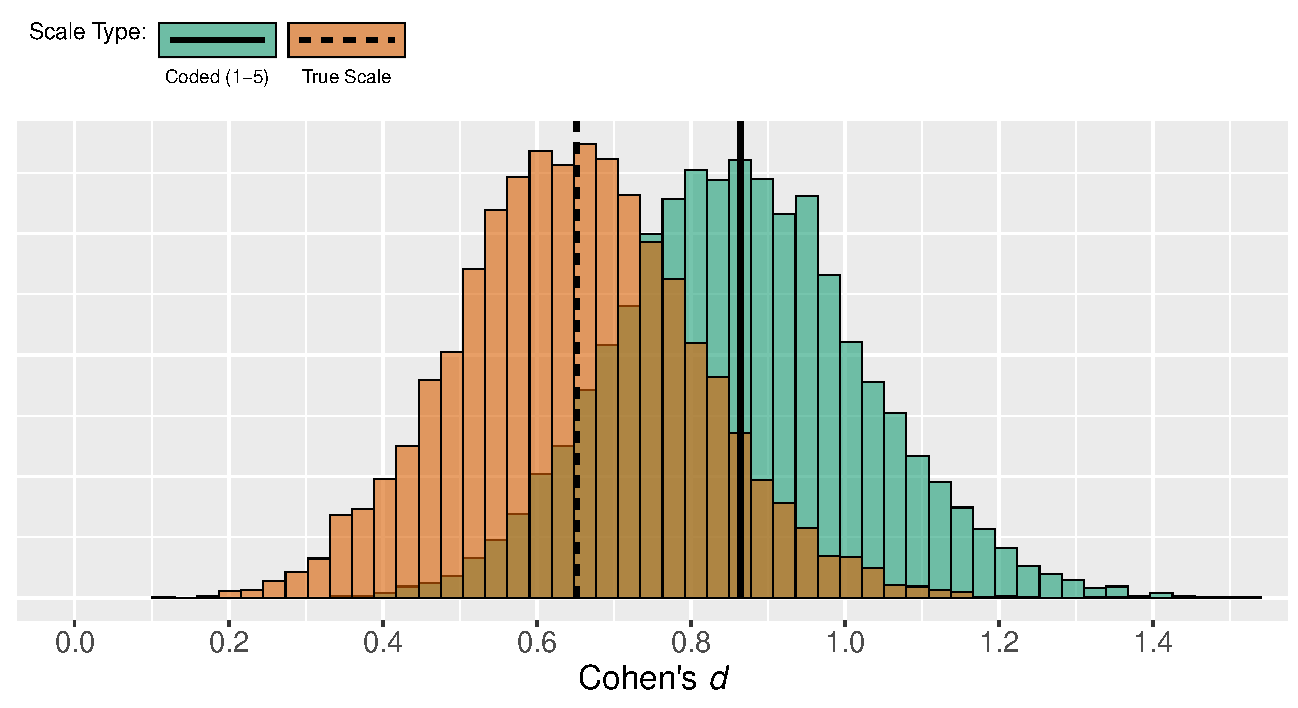
\includegraphics[width = \textwidth]{data/ordinal-effect-sim/ord_vs_int_effect.pdf}
\caption{Results from 10,000 simulated experiments comparing effect size estimates using Cohen’s \textit{d} based on Likert-scale values versus ``true'' exponentially scaled discomfort values. Although both scales preserve ordinal ranking, the unequal intervals in the true values reveal that the Likert-based \textit{d} consistently overestimates the effect size. Black horizontal lines indicate the mean Cohen’s \textit{d} for each scale type. This highlights how treating ordinal data as interval can distort results—like mistaking shoe leather for sausage.
Simulation code available at: \url{https://github.com/statistical-grimoire/book/tree/main/data/ordinal-effect-sim}}
\label{fig:ord_vs_int_effect}
\end{figure}

In this vein, it is worth noting that alternative effect size measures designed for ordinal data—such as Cliff’s delta ($\delta$)—are not susceptible to this distortion. Because Cliff’s $\delta$ relies only on order information, it produces equivalent results whether calculated from the Likert scores or the true discomfort values. In other words, when the tool matches the scale, the message stays consistent.

Because of these issues, Stevens and others attempted to prescribe which statistical methods were appropriate for each type of measurement scale to help researchers avoid making precisely these kind of mistakes \parencite{Robinson1965, Senders1958, Stevens1946}. However, that endeavour—and Stevens’ broader framework—has not gone unchallenged.

One common criticism is that his classification system is not as clear-cut as it initially appears. Many real-world variables seem to occupy a gray area. Take intelligence (I.Q.) scores, for example: while technically ordinal, they are often treated as though they possess interval properties. Researchers frequently assume that differences in I.Q. scores reflect meaningful psychological differences, even though the scale may not meet the strict criteria required for interval measurement.\footnote{This is not to suggest that differences between IQ scores \textit{do} or \textit{do not} reflect meaningful psychological differences—only that some researchers proceed as though they do.} 

Additionally, many statistical procedures that theoretically require interval or ratio-level data often yield results similar to those produced by ordinal methods when applied to ordinal-scale data \parencite{Baker1966}. This robustness has led some to argue that, in practice, violating scale assumptions may not always lead to catastrophic errors—at least not when the primary concern is \textit{statistical significance} (e.g., p-values). However, this reassurance comes with important caveats:

\begin{itemize}
    \item The consequences of misusing statistical methods can be more serious in high-stakes contexts or when findings are generalized beyond their original scope.
    \item The apparent robustness often vanishes when we move beyond \textit{p}-values to other statistics—such as Cohen’s \textit{d}—which can be heavily distorted by inappropriate assumptions about scale.
\end{itemize}

Some critics go even further, questioning whether there is any necessary connection at all between level of measurement and the validity of a statistical technique \parencite{Gaito1980}. This is arguably true—again—if the only statistic you care about is the \textit{p}-value. Others warn that strict adherence to Stevens’ taxonomy may encourage a kind of statistical ``mindlessness,'' where researchers rely on rigid checklists instead of thoughtful judgment.\footnote{This is an odd complaint, as it seems to assume that, had Stevens kept quiet, researchers would have spontaneously developed better judgment on their own. Still, the concern isn’t entirely without merit. Any framework, however well-intentioned, can be misapplied as dogma. And when tools like measurement scales are treated as gospel—especially by novices—they risk crowding out the deeper, more nuanced reasoning that good statistical practice demands.}

The debate over Stevens’ framework is long-standing, and many critiques are directed less at his core principles than at overly simplistic—or at times uncharitable—interpretations of them \parencite[see][for a summary]{ZandScholten2009}. Yet despite the criticism, Stevens’ central insight is difficult to dispute: researchers must remain mindful of how the scale of measurement can influence both the validity and the interpretation of statistical conclusions.

But the story does not end there. The idea of measurement scales is just one piece of a larger field known as Measurement Theory, which in turn sits within an even broader philosophical landscape that includes competing frameworks such as operationalism, realism, and information theory, to name a few. As fascinating (and important) as these topics are, this book is not primarily concerned with the philosophy of measurement. The discussion so far has been driven by pragmatism: in the context of doing research, Stevens’ taxonomy remains genuinely useful for thinking about data and informing analytic decisions.

Stevens gave us a practical and widely adopted classification system—but in the eyes of the most rigorously developed modern theory of measurement, \textit{Representational Measurement Theory} \parencite[RMT;][]{Luce2001}, his framework does not quite qualify as real measurement. From the RMT perspective, Stevens’ definition is too loose, and some of his scales—nominal and ordinal—do not meet the criteria for genuine measurement at all. For RMT, assigning numbers is not enough; measurement must involve assigning numbers that preserve the structure of the empirical world.

So, Stevens’ scales are not so much wrong as they are just incomplete. They provide a helpful, practical way to classify data types and choose appropriate methods, but they do not offer a rigorous foundation for what measurement truly means. You can (and should) still use them—just do not treat them as the final word.

Think of it this way: Stevens’ framework is like Newtonian physics—practical, useful, and perfectly adequate for most everyday purposes (including landing on the Moon). But just as Newton’s laws break down at relativistic speeds or near black holes—where Einstein’s theory is needed—Stevens’ model breaks down when we start asking deeper questions about the nature of measurement. In that analogy, RMT is Einsteinian: more precise, more demanding, and more accurate at the theoretical edges (but also more complex).

One especially intriguing development within this more rigorous framework of RMT is additive conjoint measurement, which demonstrates that, under certain conditions, meaningful interval-level representations can be constructed from purely ordinal data—so long as specific axioms are satisfied. This has powerful implications for the social sciences, where directly measurable quantities are rare, but ordinal judgments (like rankings or preferences) are common. In short: with the right structure, even simple orderings can yield valid and mathematically rich measurements.

\section{Other Distinctions Between Variables}

Variables are not only distinguished by their scale of measurement; they can also be more broadly categorized as either \textit{qual}itative or \textit{quant}itative. A \gls{qualitative variable} represents non-numeric characteristics or categories. These categories may be ordered (e.g., letter grades) or unordered (e.g., handedness), but they should always be mutually exclusive—that is, each observation should fall into one and only one category. For instance, a person cannot be both left-handed and right-handed simultaneously; if such a case exists, it necessitates a distinct category (e.g., ambidextrous). In practice, qualitative variables serve to classify observations into discrete groups, which is why the terms qualitative variable and categorical variable are often used interchangeably. Accordingly, it should be clear that any variable measured on a nominal or ordinal scale would also be considered qualitative in nature.\label{sec:qual_var}

A \gls{quantitative variable} tells you something about how much there is of something—it deals in actual numbers that represent real amounts or magnitudes. Unlike qualitative variables, which categorize or rank observations, quantitative variables support meaningful arithmetic operations like addition and subtraction. They are always measured on an interval or ratio scale and can be either discrete (e.g., number of siblings) or continuous (e.g., temperature, height).\label{sec:quant_var}

\begin{table}[htb]
\centering
\resizebox{\textwidth}{!}{%
%\begin{tabular}{l|l|p{5cm}|p{4cm}}
\begin{tabular}{l|l|>{\raggedright\arraybackslash}m{5cm}|>{\raggedright\arraybackslash}m{4cm}}
\toprule
\textbf{Variable} & \textbf{Scale} & \textbf{Description} & \textbf{Examples} \\
\midrule
\hyperref[sec:qual_var]{Qualitative} (Categorical) & \cellcolor{gray!10}{\hyperref[sec:nominal]{Nominal}} & \cellcolor{gray!10}{Categories with no inherent order.} & \cellcolor{gray!10}{Handedness, Eye colour, Species} \\
 & \hyperref[sec:ordinal]{Ordinal} & Values with a meaningful order, but differences between values are indeterminate. & Letter grades, Likert-scale ratings, Percentile ranks \\
 \midrule
\hyperref[sec:quant_var]{Quantitative} (Numerical) & \cellcolor{gray!10}{\hyperref[sec:interval]{Interval}} & \cellcolor{gray!10}{Numeric values with equal spacing, but no true zero} & \cellcolor{gray!10}{Temperature in Celsius, Calendar Years} \\
 & \hyperref[sec:ratio]{Ratio} & Numeric values with equal spacing and a meaningful zero & Height, Weight, Reaction time \\
\bottomrule
\end{tabular}
}
\caption{Summary of variables and corresponding measurement scales}
\label{tab:var_sum}
\end{table}


A \gls{discrete variable} is one that takes on a finite number of values (e.g., the number of cells in a slice of brain tissue) or a countably infinite set of values (e.g., the set of odd numbers). In other words, discrete variables are countable using the natural numbers: 1, 2, 3, and so on. Calling a variable ``discrete'' means there are no possible values in between—the values are separate, distinct steps. For example, it does not make sense to count 12.5 brain cells. Even if, under a microscope, a cell appears partially missing, you must decide whether to count it as a whole cell or not at all.

By contrast, if it makes sense to talk about values between any two measurements, the variable is no longer discrete—it is continuous. A \gls{continuous variable} can, at least in theory, take on any numeric value within a given range. These variables have uncountably infinite possibilities. For example, temperature is a continuous variable. Between 20°C and 21°C, there are infinitely many possible values—like $20.1^\circ$C, $20.01^\circ$C, or $20.0001^\circ$C. No matter how small the interval, there is always another possible value in between. Of course, in practice, temperature often appears discrete—especially when measured with a thermometer that rounds to the nearest degree. But this discreteness is an illusion caused by the limitations of our measuring tools. In reality, temperature varies continuously; it is our instruments (and our finite senses) that force us to round or approximate.

Bringing this back to scales of measurement: any variable measured on an interval or ratio scale is, by definition, also a quantitative variable.

